\chapter{Les outils de Scans}
\label{chap:BDD}

Lors d'une attaque, le scan est une obligation pour savoir où attaquer la cible. En effet, que ce soit pour découvrir les ports ouverts ou pour savoir quelles vulnérabilités sont présentes, nous aurons besoin d'un scanneur. Nous vous présenterons dans un premier temps un scanneur de port qui sera Nmap. Puis nous allons vous présenter l'outil Nikto pour ce qui est du scan de vulnérabilités d'un site Web.

\section{Nmap}
\subsection{Présentation de Nmap}
Nmap est un utilitaire permettant de scanner les ports ouverts d’une machine ou d’un ensemble de machines présentes dans un même réseau. Chaque programme voulant émettre sur le réseau va devoir sortir de son hôte. Chacun d’eux va se voir alors attribuer une porte pour sortir et qui devra rester ouverte tant qu’ils voudront émettre. Ces portes sont les ports ouverts d’une machine. En trouvant ces ports, Nmap se rend comme l’élément essentiel d’une attaque réseau. En effet, sans cette analyse, nous serions incapable de trouver un chemin d’attaque à moins d’avoir une chance inouïe. C’est pourquoi nous allons utiliser cet utilitaire pour résoudre nos CTFs.



\subsection{Fonctionnement de Nmap}
Tout d’abord, Nmap peut être utilisée en lui renseignant qu’une adresse IP sans option comme ceci :
\begin{figure}[htp!]
  \centering
  \setlength\figureheight{7cm}
  \setlength\figurewidth{9cm}
  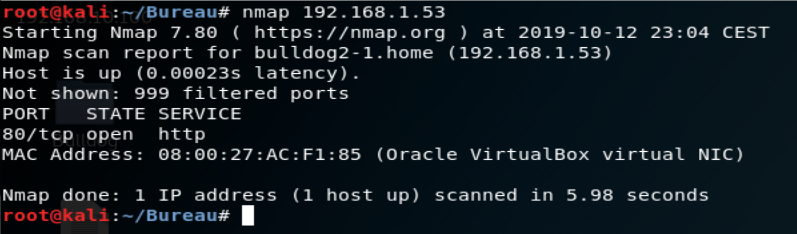
\includegraphics[width=0.7\textwidth]{oui/Screens/nmap/justeip.PNG}
  \caption{Utilisation de nmap sans options}
  \label{fig:courbe-tikz}
\end{figure}

\newpage
Cette commande intuitive et rapide nous permet d’obtenir le port ouvert ainsi que le protocole qui lui est associé. Cependant, il serait intéressant pour une futur exploitation de faille, d’obtenir le nom du \textbf{S}erveur web ainsi que sa \textbf{V}ersion. C’est pourquoi nous allons appliquer l’argument ‘ -sV ‘ :
\begin{figure}[htp!]
  \centering
  \setlength\figureheight{7cm}
  \setlength\figurewidth{9cm}
  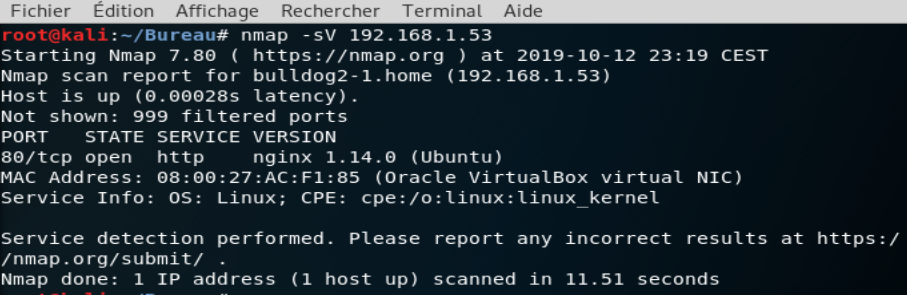
\includegraphics[width=1\textwidth]{oui/Screens/nmap/-sV.PNG}
  \caption{Ajout de l'opton -sV}
  \label{fig:courbe-tikz}
\end{figure}

Le CTF analysé ici utilise un serveur web nginx de version $1.14.0$. Nous ne pouvons que vous conseiller de garder ce type d’informations dans un bloc-note tout au long d’une attaque.\\
Nous pouvons à partir de ce résultat se demander comment Nmap récupère les informations concernant la version des serveurs. Tout d'abord, Il faut savoir que cet outil travaille sur deux base données : une pour les ports et une autre pour les versions des logiciels et serveurs. Pour ce qui est des ports, la base de données se nomme 'nmap-service' et est visualisable via ce lien :\\
https://svn.nmap.org/nmap/nmap-services\\
La base de données pour les versions est 'nmap-service-probes' :\\
https://svn.nmap.org/nmap/nmap-service-probes\\
Afin de comprendre comment Nmap exploite ces dictionnaires, nous avons réécrit en Python un programme scannant les ports d'un serveur Samba et affichant la version du protocole utilisé. Il faut savoir avant d'observer le programme que Nmap utilise des regex afin de comparer la réponse envoyée par le serveur et ainsi obtenir la version. Voici notre programme :

\begin{figure}[htp!]
  \centering
  \setlength\figureheight{7cm}
  \setlength\figurewidth{9cm}
  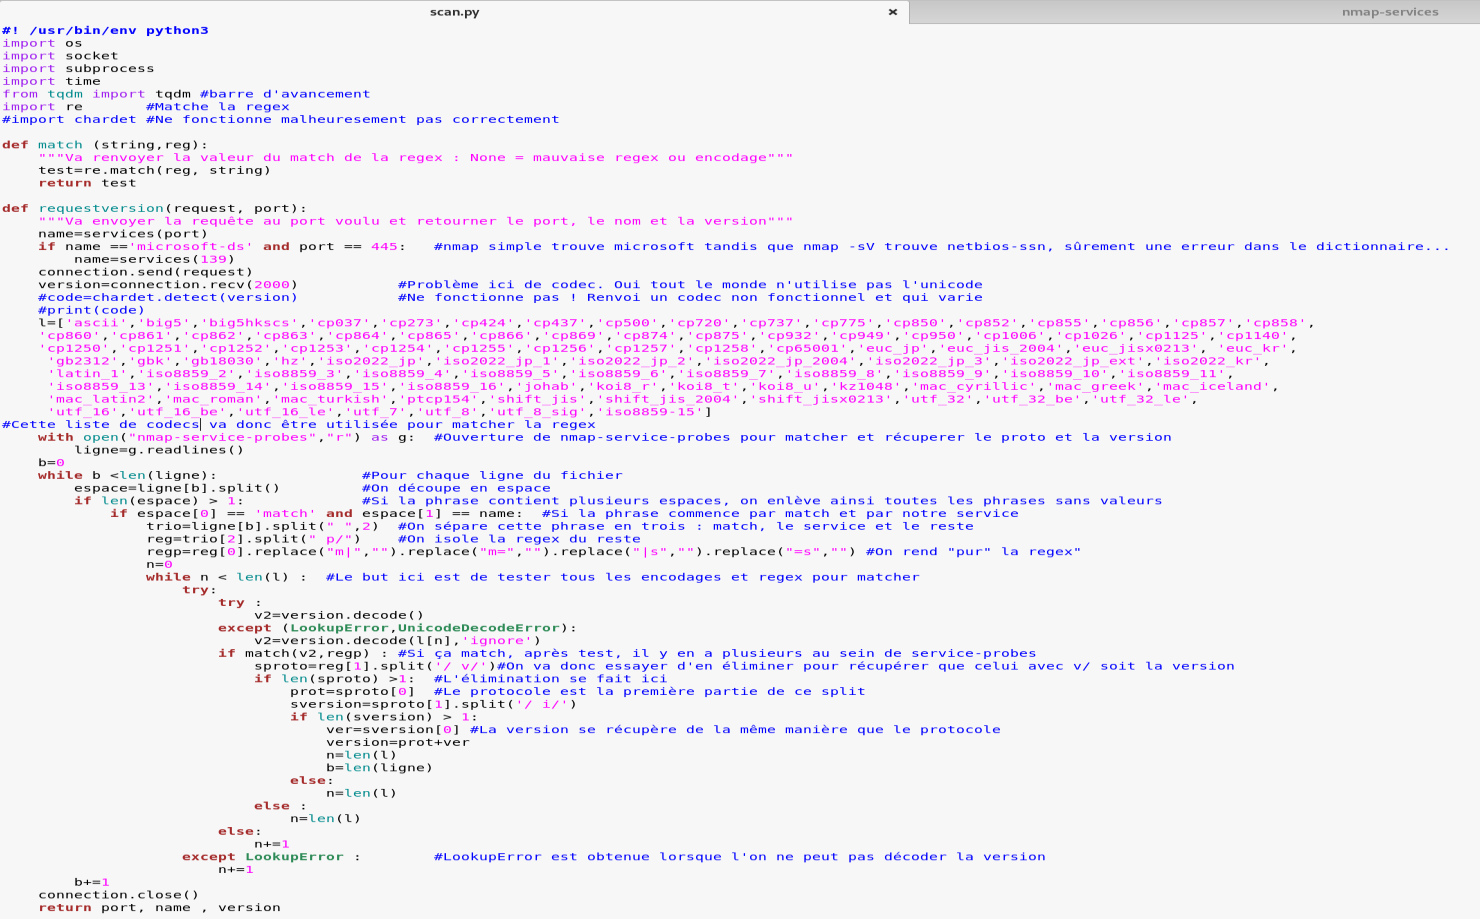
\includegraphics[width=0.9\textwidth]{oui/Screens/nmap/Part1.PNG}
  \caption{Scanneur Samba partie 1}
  \label{fig:courbe-tikz}
\end{figure}

\begin{figure}[htp!]
  \centering
  \setlength\figureheight{7cm}
  \setlength\figurewidth{9cm}
  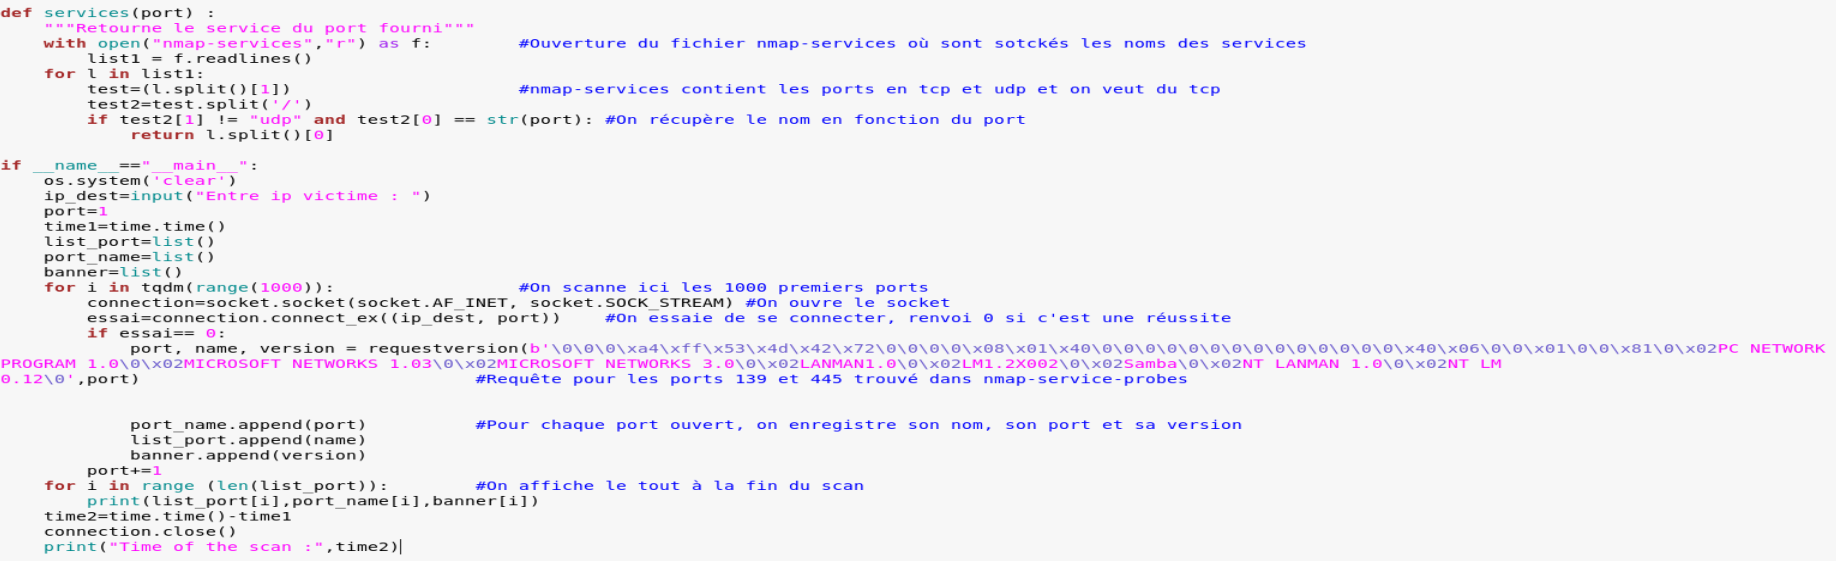
\includegraphics[width=0.9\textwidth]{oui/Screens/nmap/Part2.PNG}
  \caption{Scanneur Samba partie 2}
  \label{fig:courbe-tikz}
\end{figure}

\newpage
Lors de son exécution, on voit apparaître le nom du service, son port ainsi que sa version. On peut comparer son exécution avec Nmap :

\begin{figure}[htp!]
  \centering
  \setlength\figureheight{7cm}
  \setlength\figurewidth{9cm}
  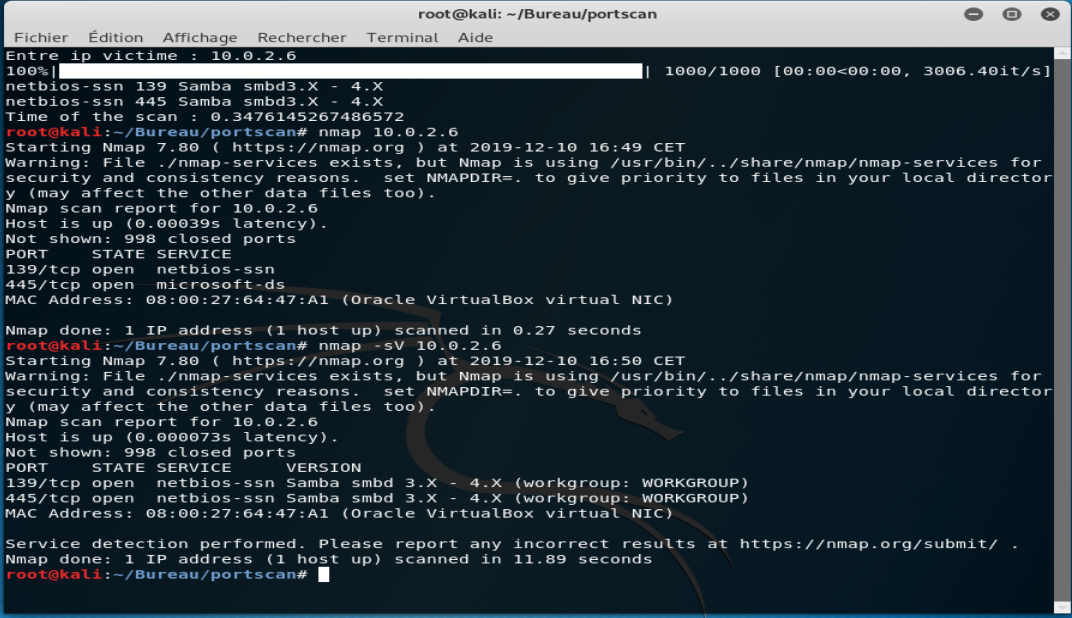
\includegraphics[width=0.9\textwidth]{oui/Screens/nmap/Result.PNG}
  \caption{Scanneur Samba}
  \label{fig:courbe-tikz}
\end{figure}

\newpages
On remarque que notre programme affiche les résultats en 0.34 secondes contre en 11.89 secondes avec Nmap. On suppose que Nmap réalise d'autres calculs en arrière plan pour obtenir une vérification de la version. Voici une différence entre notre programme et Nmap au niveau de Wireshark :

\begin{figure}[htp!]
  \centering
  \setlength\figureheight{7cm}
  \setlength\figurewidth{9cm}
  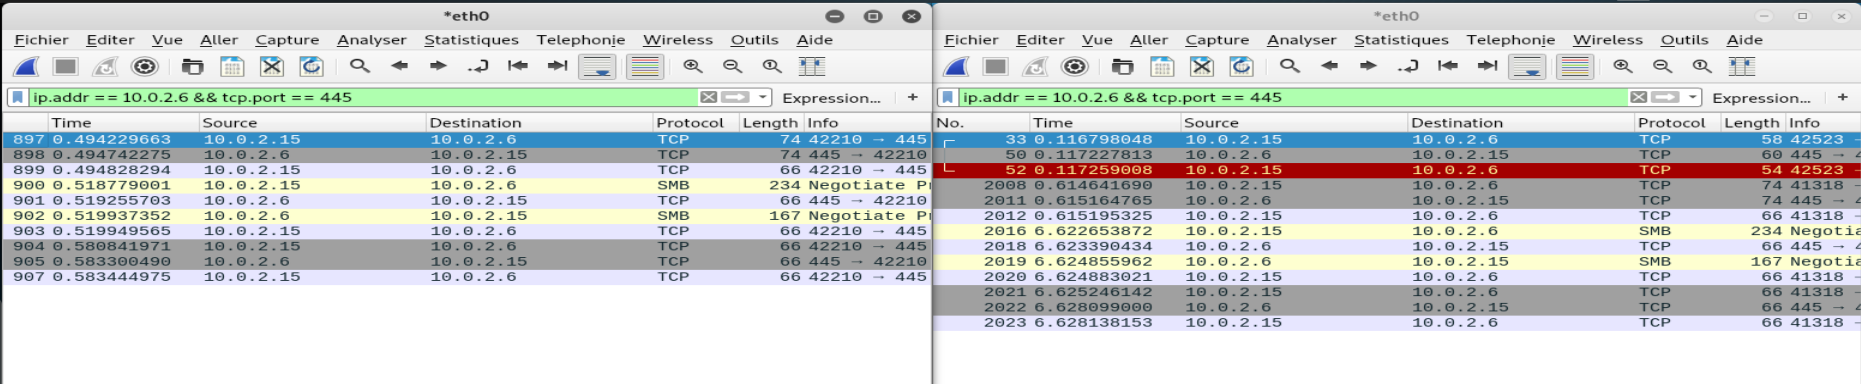
\includegraphics[width=0.9\textwidth]{oui/Screens/nmap/wireshark_prog.PNG}
  \caption{Gauche : Python et Droite : Nmap}
  \label{fig:courbe-tikz}
\end{figure}

En effet, Nmap réalise un RST après avoir testé l'ouverture du port pour réinitialiser la connexion du socket. C'est alors après qu'il lance une séquence d'initialisation TCP (SYN, SYN ACK, ACK) afin d'envoyer sa requête au serveur via le protocole SMB. Ce dernier lui renvoie une valeur incompréhensible par l'homme qu'il faut décoder pour le matcher avec la base de données de Nmap. C'est ainsi que Nmap opère pour récupérer la version du protocole utilisée.


\newpage
Maintenant que nous avons vu comment utiliser basiquement Nmap, nous pouvons nous demander comment fonctionne cet utilitaire. En effet, il est obligé de faire des requêtes sur tous les ports en utilisant le protocole ICMP, IP, TCP et UDP. Cet utilitaire utilise donc les couches 3 et 4 du modèle OSI.\\
Cependant, en émettant toutes ses requêtes, Nmap laisse des traces :
\begin{figure}[htp!]
  \centering
  \setlength\figureheight{7cm}
  \setlength\figurewidth{9cm}
  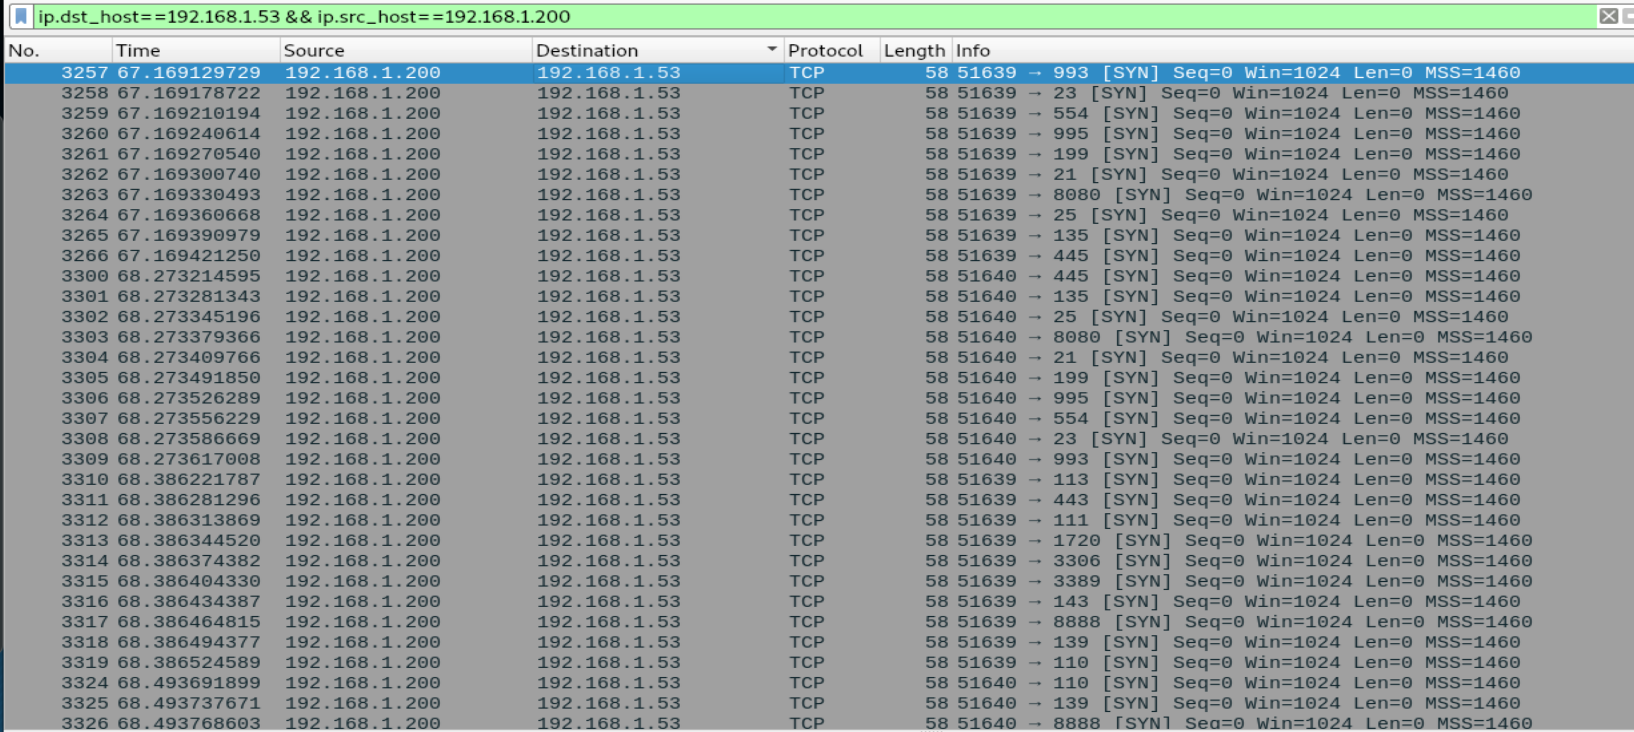
\includegraphics[width=0.85\textwidth]{oui/Screens/nmap/Wiresharkhypervisible.PNG}
  \caption{Scan avec wireshak}
  \label{fig:courbe-tikz}
\end{figure}

Nous allons donc voir comment éviter de nous faire "trop" repérer sur le réseau.\\
Dans un premier temps, nous pouvons fragmenter nos paquets avec l’option ‘ -f ‘ :
\begin{figure}[htp!]
  \centering
  \setlength\figureheight{7cm}
  \setlength\figurewidth{9cm}
  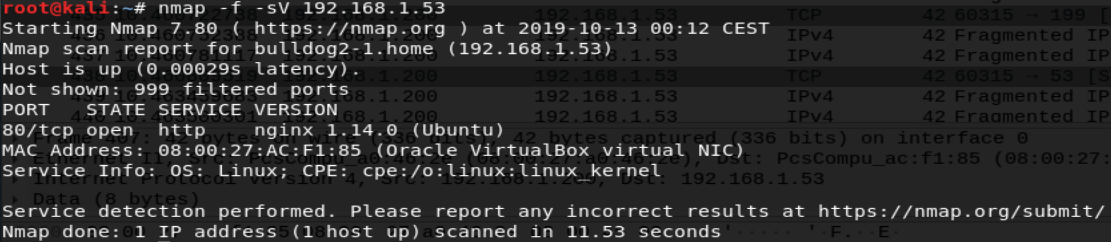
\includegraphics[width=1\textwidth]{oui/Screens/nmap/-f.PNG}
  \caption{Ajout de l'option -f}
  \label{fig:courbe-tikz}
\end{figure}

Cette option va fragmenter nos paquets pour les éparpiller sur le réseau et ainsi ne pas indiquer tout de suite que nous scannons le port 80 comme avant :
\begin{figure}[htp!]
  \centering
  \setlength\figureheight{7cm}
  \setlength\figurewidth{9cm}
  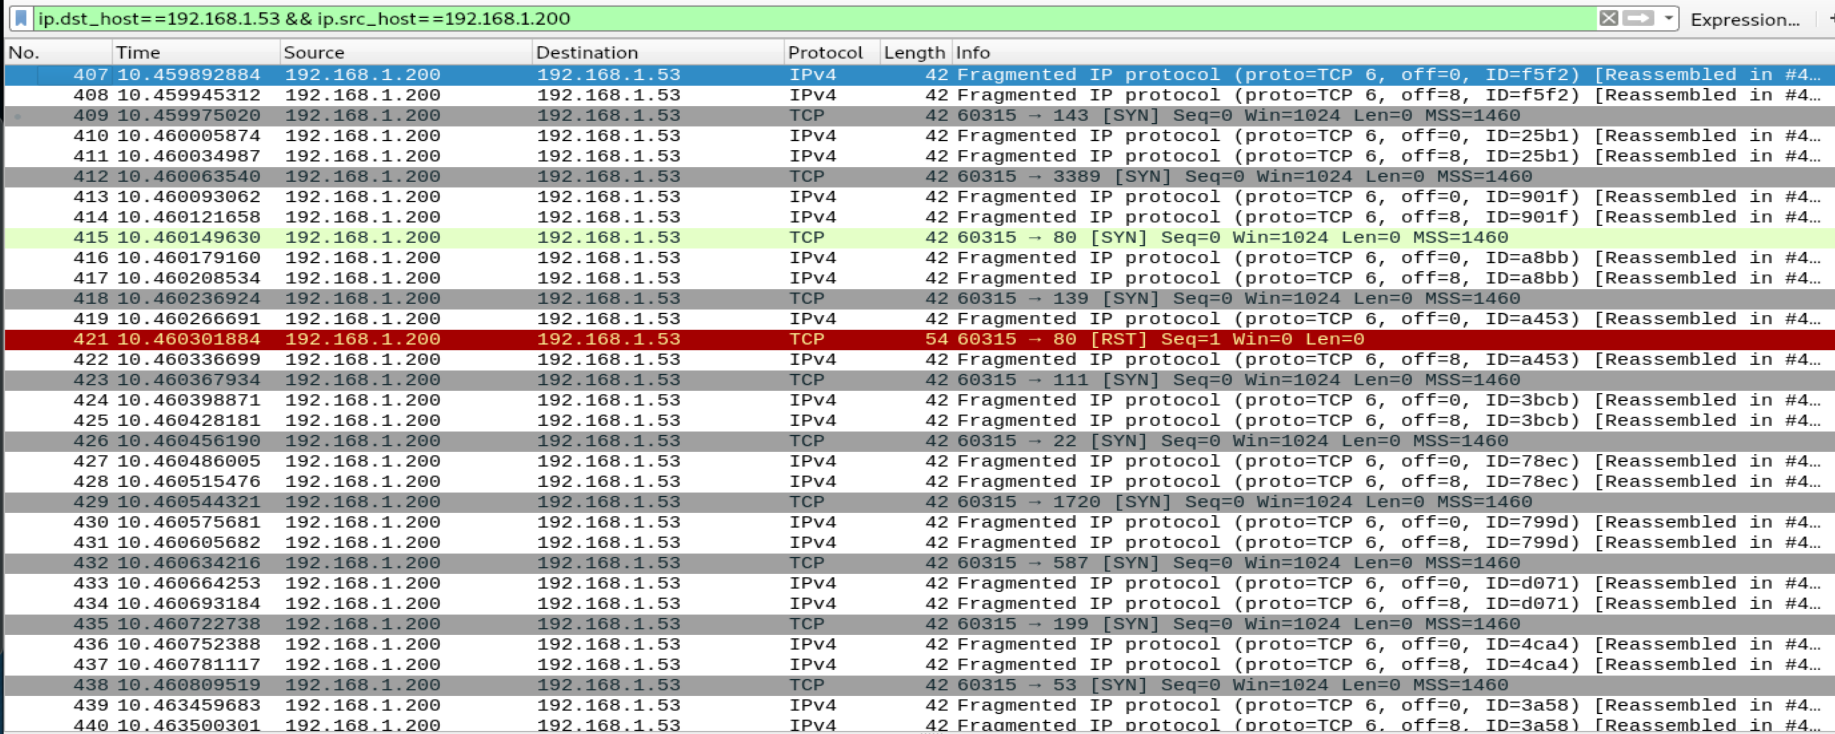
\includegraphics[width=0.75\textwidth]{oui/Screens/nmap/Wireshark-f-Copie.PNG}
  \caption{Scan avec wireshak en ajoutant l'option -f}
  \label{fig:courbe-tikz}
\end{figure}

\newpage
La capture Wireshark ci-dessus nous montre qu’en fragmentant nos paquets, nous utilisons le protocole IP et TCP. De plus, cette fragmentation permet de noyer le scan de ports ( les [SYN] ) et d’outrepasser un firewall. En effet, de vieux firewalls peuvent avoir des failles comme celles de la fragmentation. Ces derniers étaient incapables de s’en occuper donc les laissaient passer. Cependant, les programmeurs ont résolus le problème donc cette faille n’est plus exploitable sur les nouveaux firewalls. C'est pour cette raison que nous n'allons pas détailler cette méthode fragmentation.\\
Comme nous l'avons vu, Nmap se fait passer un client lambda via ses requêtes. Cependant, il envoie par défaut un nombre de requêtes par seconde qui n'est pas réalisable par un humain. Cette vitesse d'envoi par défaut est le T3 qui scanne un port toutes les 16 ms ce qui provoque une alarme chez les firewalls. Voici un tableau qui répertorie la vitesse de scan pour un port :

\begin{figure}[htp!]
  \centering
  \setlength\figureheight{7cm}
  \setlength\figurewidth{9cm}
  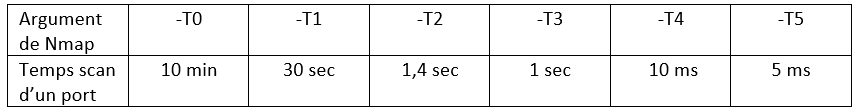
\includegraphics[width=1\textwidth]{oui/Screens/nmap/tableau.PNG}
  \caption{Tableau vitesse de scan}
  \label{fig:courbe-tikz}
\end{figure}

Les valeurs de ce tableau peuvent varier en fonction du processeur, de la quantité de RAM et du débit sur le réseau. On peut remarquer le T0 et le T1 peuvent se faire passer pour un humain et seront donc utilisés pour être indétectables par les firewalls. Cependant, ce scan, même en T1, risque de prendre énormément de temps. Si on pose le calcul théorique, notre scan en T1, le plus rapide des indétectables, prendrai 50 heures pour scanner les mille premiers ports.
 

\newpage
Nous commençons à avoir une belle couverture de nos traces sur le réseau. Mais nous allons essayer de faire mieux en usurpant une adresse MAC du réseau pour passer pour un autre :

\begin{figure}[htp!]
  \centering
  \setlength\figureheight{7cm}
  \setlength\figurewidth{9cm}
  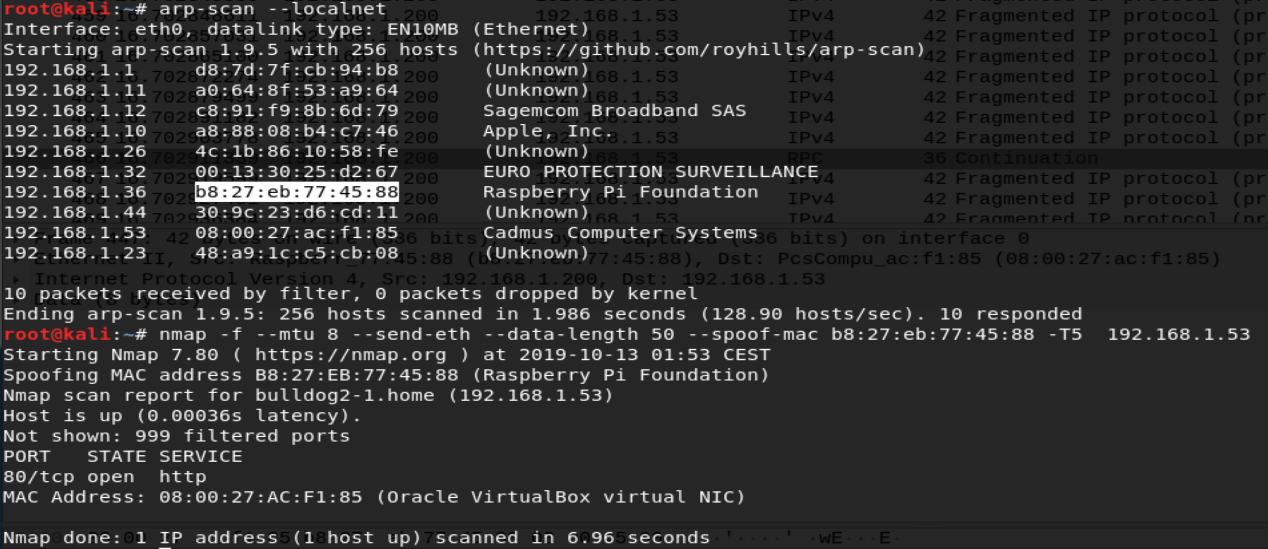
\includegraphics[width=1\textwidth]{oui/Screens/nmap/spoof-mac.PNG}
  \caption{Usurpation d'adresse MAC}
  \label{fig:courbe-tikz}
\end{figure}

L’option ‘ --spoof-mac ‘ nous permet de remplacer notre adresse MAC par celle renseignée en argument de l’option. Voici comment réagit Wireshark face à ce changement :

\begin{figure}[htp!]
  \centering
  \setlength\figureheight{7cm}
  \setlength\figurewidth{9cm}
  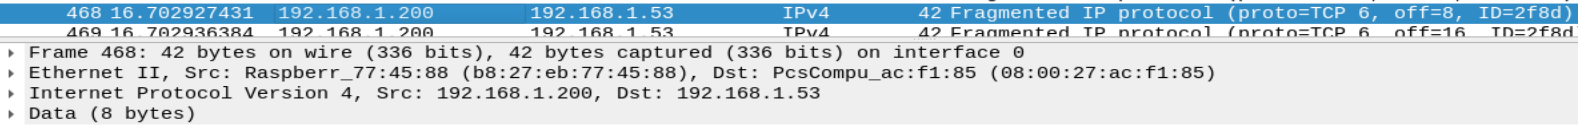
\includegraphics[width=1\textwidth]{oui/Screens/nmap/Wiresharkspoofmac.PNG}
  \caption{Wireshark usurpation MAC}
  \label{fig:courbe-tikz}
\end{figure}

Allons encore plus loin en usurpant l’IP d’une autre machine :

\begin{figure}[htp!]
  \centering
  \setlength\figureheight{7cm}
  \setlength\figurewidth{9cm}
  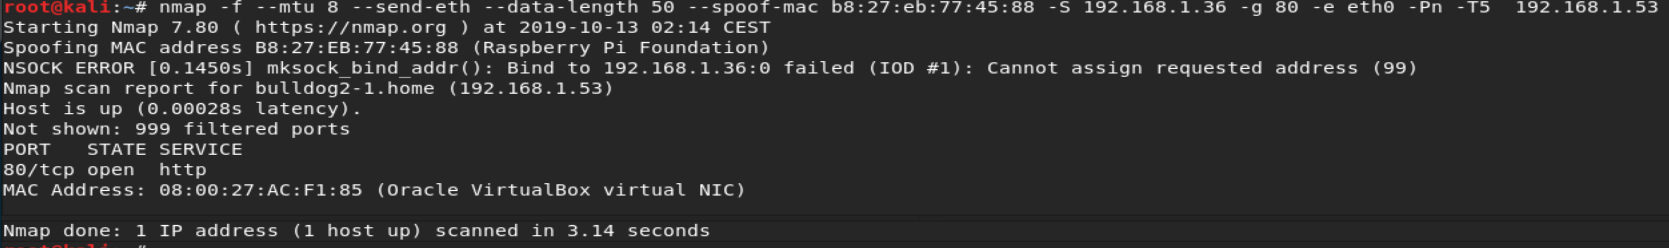
\includegraphics[width=1\textwidth]{oui/Screens/nmap/spoofipetmac.PNG}
  \caption{Usurpation MAC et IP}
  \label{fig:courbe-tikz}
\end{figure}

De cette manière, nous avons pu faire simuler un Nmap à partir du Raspberry présent sur le réseau. L’option ‘ -S ‘ permet d’associer une IP source au paquet. Cette option doit être accompagnée d'un ‘ -g ‘ pour lui indiquer le port de sorti ainsi que de l’option ‘ -e ‘ pour informer notre interface réseau. Nmap nous recommande d’utiliser l’option ‘ -Pn ‘ pour considérer que tous les hôtes sont en ligne.
Nous obtenons un Wireshark vide entre notre machine et la cible.
Si nous observons une capture de trafic entre le Raspberry et la cible :

\begin{figure}[htp!]
  \centering
  \setlength\figureheight{7cm}
  \setlength\figurewidth{9cm}
  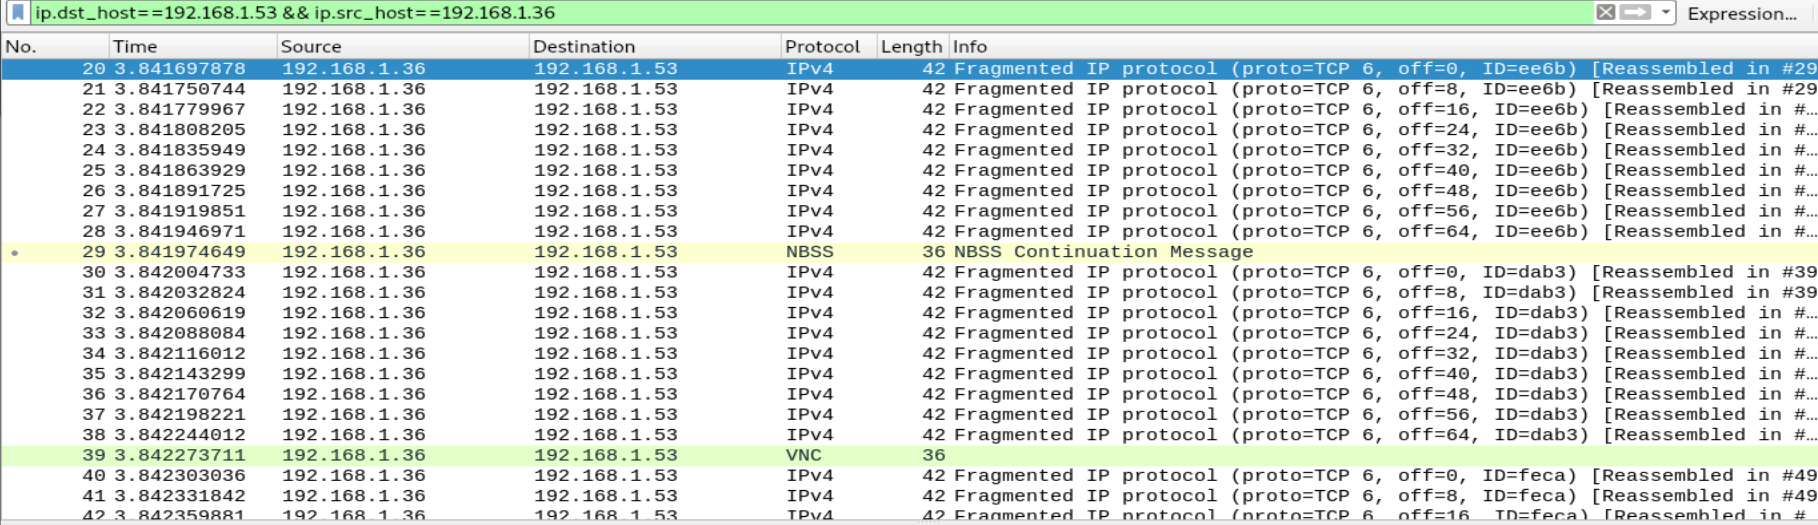
\includegraphics[width=1\textwidth]{oui/Screens/nmap/Wiresharkusurpe.PNG}
  \caption{Wireshark usurpation MAC et IP}
  \label{fig:courbe-tikz}
\end{figure}

\noindent Nos paquets fragmentés sont bien envoyés entre les deux et nous recevons la réponse de notre scan sans être impliqué dans la ‘discussion’.
Notre scan est alors une réussite.\\
Mais comment avons nous pu récupérer ces informations sans être présent dans les discutions ? Comme nous l'avons vu plus haut, l'option '-e ' a pour but d'informer Nmap de faire sortir et entrer les informations via un port que l'on ouvre sur notre machine. Via ce procédé, notre interface va envoyer et recevoir les paquets échangés entre la machine cible et celle usurpée.  Ainsi, nous nous plaçons tel un proxy et nous récupérons en ‘man-in-the-middle’ les informations sans être vu. Il y a plusieurs types d’attaques ‘man-in-the-middle’. Ici, nous utilisons le type d’attaque ‘ARP spoofing’ en usurpant les adresses d’une machine dans le même réseau que la machine cible et en forçant les communications à transiter par notre machine virtuelle en se faisant passer pour un relais.

\subsection{Réaction d'un firewall Stormshield face à Nmap}

Au cours de cette présentation de Nmap, nous n'avions aucune sécurité présente entre la l'attaquant et la cible. Nous allons donc réaliser une attaque d'un réseau à l'autre avec pour routeur un firewall Stormshield. Un firewall est un équipement physique ou non, qui permet de sécuriser les entrées et les sorties d'un réseau. Nous allons ici utiliser un firewall Stormshield SN210W qui est un équipement physique. Voici la topologie utilisée lors de ces essais :

\begin{figure}[htp!]
  \centering
  \setlength\figureheight{7cm}
  \setlength\figurewidth{9cm}
  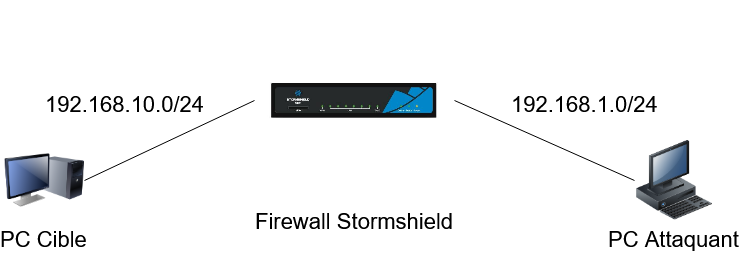
\includegraphics[width=1\textwidth]{oui/Screens/nmap/FirewallDiagram.png}
  \caption{Topologie}
  \label{fig:courbe-tikz}
\end{figure}

\newpage
Nous avons utilisé la configuration d'usine du firewall afin d'avoir un point de vue objectif face à Nmap. Au cours de ces essais, nous allons utiliser une attaque témoin qui sera l'attaque sans option de Nmap. Nous pouvons alors regarder les logs du firewall à la suite de cette attaque :

\begin{figure}[htp!]
  \centering
  \setlength\figureheight{7cm}
  \setlength\figurewidth{9cm}
  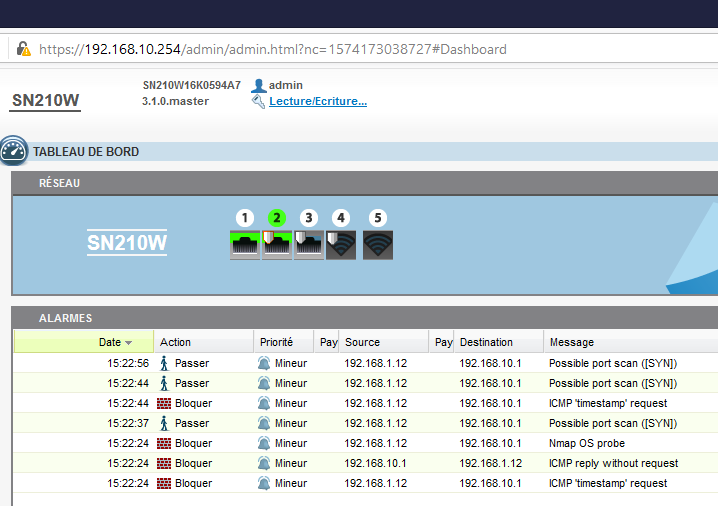
\includegraphics[width=0.9\textwidth]{oui/Screens/nmap/stormshield/alarme_nmap_base.PNG}
  \caption{Log Stormshield face à un Nmap sans option}
  \label{fig:courbe-tikz}
\end{figure}

\newpage
Le firewall détecte très facilement la présence de Nmap et bloque les requêtes ICMP faites par l'attaquant. Cependant, nous pouvons observer une faille au niveau des requêtes SYN car le firewall les laisse passer. Pour confirmer cette théorie, nous avons fais une requête de versions qui s'est aboutie en 152,93 secondes. Nous ne pouvons pas afficher les alarmes tellement les firewall en a déclaré. Cependant, encore une fois, Nmap était détecté et les SYN sont passés. Nous allons donc forcer Nmap à effectuer un scan en utilisant que des SYN avec la comande '-sS' :

\begin{figure}[htp!]
  \centering
  \setlength\figureheight{7cm}
  \setlength\figurewidth{9cm}
  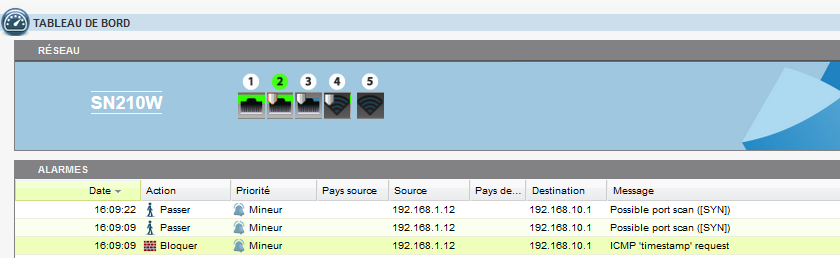
\includegraphics[width=0.9\textwidth]{oui/Screens/nmap/stormshield/Alarme-sS.PNG}
  \caption{Log Stormshield face à un Nmap -sS}
  \label{fig:courbe-tikz}
\end{figure}

Ce scan s'est terminé en 14,43 secondes ce qui est en moyenne plus long qu'un scan sans option. Cependant, le résultat est concluant car le firewall ne détecte plus la présence de Nmap. Nous allons procéder de la même manière afin de récupérer les versions :

\begin{figure}[htp!]
  \centering
  \setlength\figureheight{7cm}
  \setlength\figurewidth{9cm}
  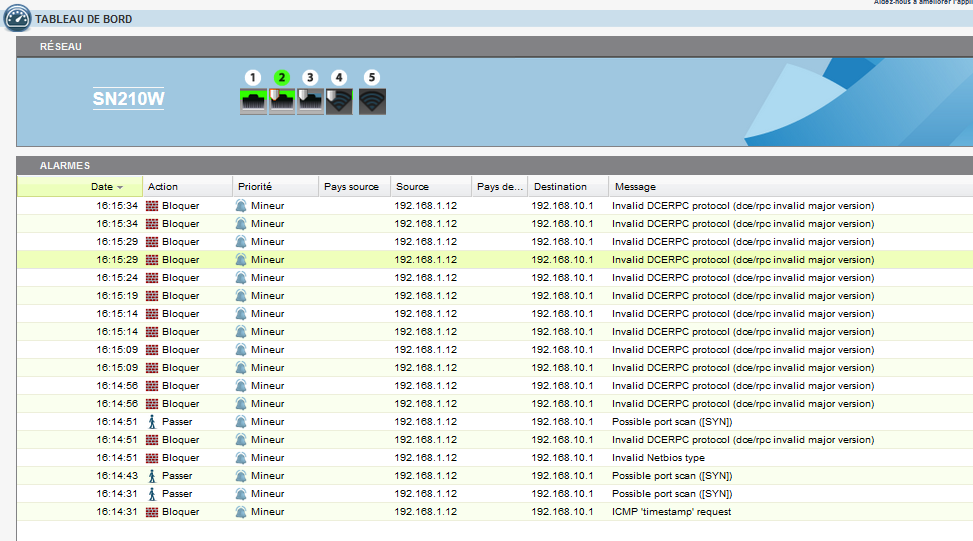
\includegraphics[width=0.9\textwidth]{oui/Screens/nmap/stormshield/result-sS-sV.PNG}
  \caption{Log Stormshield face à un Nmap -sS -sV}
  \label{fig:courbe-tikz}
\end{figure}

\newpage
Le scan s'est terminé en 63,72 secondes soit un gain de 58,33\% de temps comparé au scan de version standard. De plus, le nombre à diminué de plus de moitié, ce qui permet de les afficher ci-dessus. On peut remarquer que le plus gros nombre d'alarme se déclenche sur des requêtes DCERPC invalides. Le protocole DCE/RPC (Distributed Computing Environment /Remote Procedure Calls) permet des envois à distance comme pourrait faire un serveur Samba. Microsoft utilise énormément ce protocole pour mettre en place ses services. Or dans notre cas, la cible possède plusieurs services utilisant MS-RPC comme le montre le résultat du scan -sS -sV :

\begin{figure}[htp!]
  \centering
  \setlength\figureheight{7cm}
  \setlength\figurewidth{9cm}
  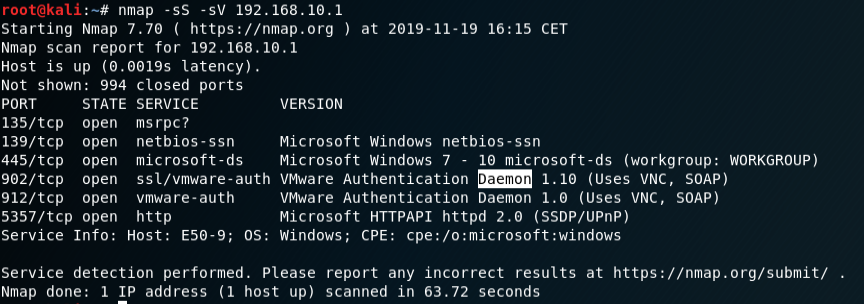
\includegraphics[width=0.9\textwidth]{oui/Screens/nmap/stormshield/commande-sS-sV.PNG}
  \caption{Nmap -sS -sV}
  \label{fig:courbe-tikz}
\end{figure}

Ceci nous montre que un ou plusieurs protocoles utilisés par Windows ne sont pas autorisés par le firewall. Certes, notre scan Nmap crée des alertes sur le firewall mais ces alertes seront presque invisibles après la configuration du Stromshield au sein d'une grande entreprise. En effet, soit l'administrateur réseau devra désactiver sur chaque ordinateur les services MS-RPC ou les autoriser sur le firewall afin de ne pas avoir d'alarmes intempestives. Etant donné le nombre de messages passant le firewall, nos messages pourront se mêler aux ceux des employés sans être vus.\\
Nous auront malheureusement du mal avec Nmap à camoufler notre IP. En effet, après avoir rajouter une machine en 192.168.1.11, nous avons réalisé un spoof IP et MAC pour attaquer notre cible. Cependant, notre firewall doit réaliser des requêtes sur le réseau bloquant ce système comme on peut le voir ci-dessous :

\begin{figure}[htp!]
  \centering
  \setlength\figureheight{7cm}
  \setlength\figurewidth{9cm}
  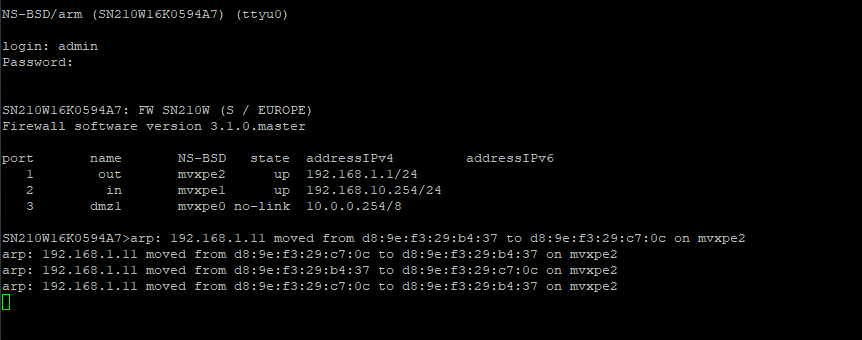
\includegraphics[width=0.9\textwidth]{oui/Screens/nmap/stormshield/screen_spoofmac.PNG}
  \caption{Spoof non fonctionnel}
  \label{fig:courbe-tikz}
\end{figure}

\newpage
Le Stromshield a écrit ceci dans sa CLI. On y comprend que le firewall fait des requêtes ARP afin de vérifier l'identité du client et annule notre spoof MAC.

\textbf{Conclusion}:\\
Nmap est un outil de scan de ports très puissant. Ce dernier a la capacité de nous faire disparaître des échanges réseaux tout en capturant les informations sur les ports de la cible.

\section{Nikto}

Lorsque les hackeurs ont pour objectif d’attaquer une cible, ils ont recours à un outil tel que Nikto afin de scanner les vulnérabilités et de passer le moins de temps possible à attaquer la cible à proprement parlé. Nikto est donc un outil permettant aux hackeurs de gagner du temps.
Nikto est un scanner de vulnérabilités web écrit en Perl et sous licence GPL. Il va permettre de tester la sécurité de la configuration d'un serveur web (les options HTTP, les index, les potentielles failles XSS, injections SQL etc…).\\
Avant de montrer ce que peut réaliser Nikto, nous pouvons dans un premier temps revoir comment fonctionne une requête Web. Parmis les ports réservés, les serveurs Web ont pour port 80 pour l'HTTP ou 443 pour l'HTTPS. Pour comprendre le fonctionnement, nous allons analyser un échange entre un client et un serveur :

\begin{figure}[htp!]
  \centering
  \setlength\figureheight{7cm}
  \setlength\figurewidth{9cm}
  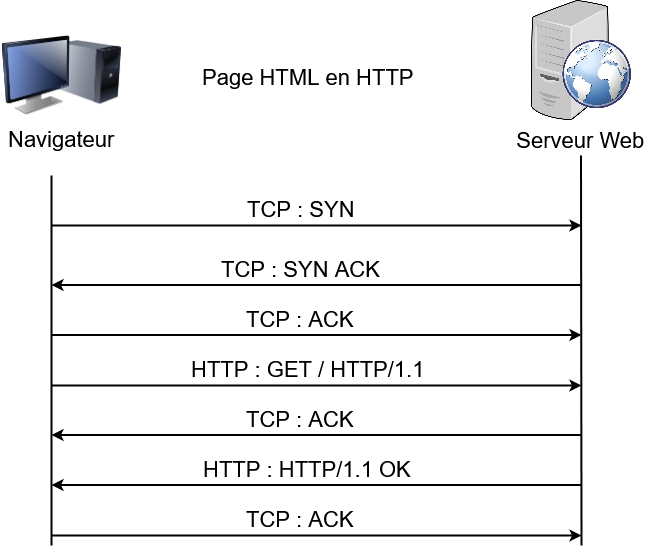
\includegraphics[width=0.7\textwidth]{oui/Screens/Nikto/wEBDiagram.png}
  \caption{Échange entre un navigateur et un serveur Web}
  \label{fig:courbe-tikz}
\end{figure}

\newpage
Comme vous pouvez le voir, le schéma ci-dessus ainsi que la capture wireshark ci-dessous montrent l'échange minimal entre un navigateur et un serveur Web afin d'obtenir une page HTML via HTTP.Une page Web n'est pas une vidéo que l'on regarde en streaming ou un appel vidéo qui utilise le protocole de transport UDP pour transmettre les paquets. En effet, lorsque nous chargeons une page Web, nous la voulons complète et sans erreurs. C'est pourquoi le protocole TCP existe. Sur notre diagramme d'échange, nous pouvons observer que le protocole TCP est présent lors des trois premiers échanges (SYN, SYN ACK, ACK). Ces échanges TCP se nomment 3-Way-Handshake, qui peut se traduire par : "les trois échanges pour se mettre d'accord sur la connexion". Il faut comprendre que après chaque échange, le protocole TCP prévoit un ACK (acquittement) pour annoncer que le paquets a été reçu sans erreurs. Maintenant que nous avons compris TCP, nous pouvons passer à la couche applicative de cet échange : le HTTP. Les envois HTTP sont directement émis par le navigateur et par le serveur Web. Ici, c'est notre navigateur qui fait une requête GET au serveur pour obtenir l'ensemble de la page Web voulue. Il existe plusieurs types de requêtes Web (GET, POST, HEAD, ...) mais seul le GET va nous intéresser car il est le plus utilisé. 

\begin{figure}[htp!]
  \centering
  \setlength\figureheight{7cm}
  \setlength\figurewidth{9cm}
  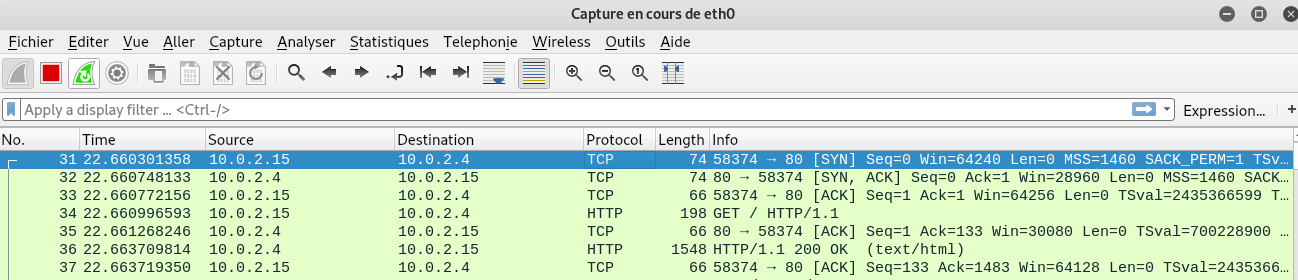
\includegraphics[width=0.7\textwidth]{oui/Screens/Nikto/wireshark1.png}
  \caption{Capture Wireshark d'un scan nikto}
  \label{fig:courbe-tikz}
\end{figure}

\newpage
Lors du scan, Nikto est capable de :\\
\textbf{- Vérifier}     si la version du serveur est obsolète ainsi que les logiciels et     modules qui sont utilisés par ce dernier. \\   
\textbf{- Scanner}     les répertoires, qui peuvent contenir des informations sensibles.\\
\textbf{- Tester}     près de 6000 fichiers potentiellement vulnérables.\\
De plus, Nikto supporte les connections SSL.

\subsection{Utilisation de Nikto}
Pour lancer un simple scan, il suffit de réaliser la commande :

\begin{figure}[htp!]
  \centering
  \setlength\figureheight{7cm}
  \setlength\figurewidth{9cm}
  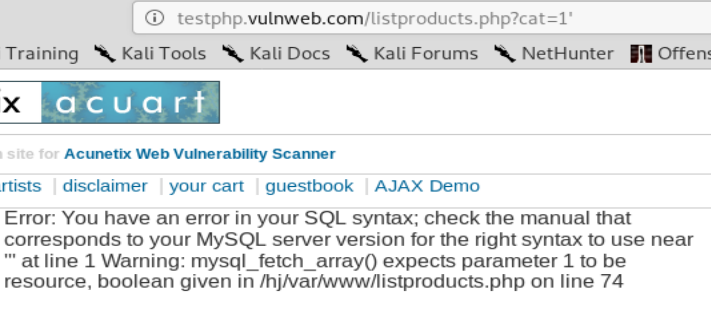
\includegraphics[width=0.8\textwidth]{oui/Screens/Nikto/1.PNG}
  \caption{Scan simple}
  \label{fig:courbe-tikz}
\end{figure}

\begin{figure}[htp!]
  \centering
  \setlength\figureheight{7cm}
  \setlength\figurewidth{9cm}
  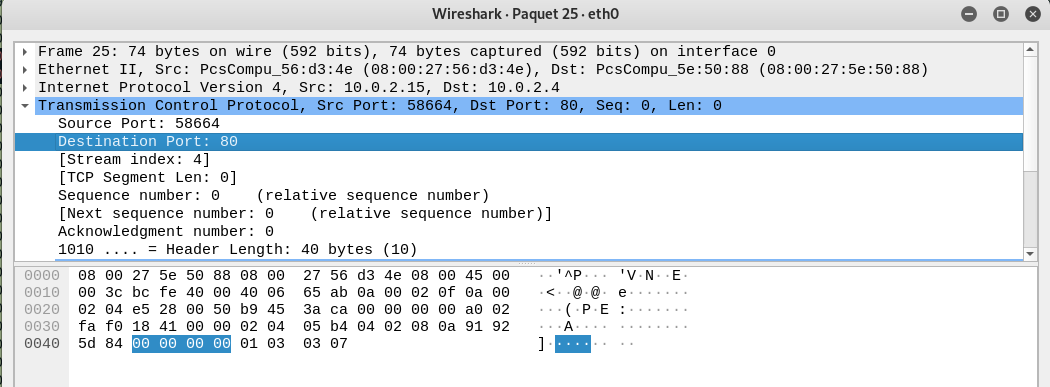
\includegraphics[width=0.8\textwidth]{oui/Screens/Nikto/wireshark3.png}
  \caption{Mise en évidence du port scanné par défaut par la commande nikto}
  \label{fig:courbe-tikz}
\end{figure}

On peut remarquer grâce à cette capture wireshark que par défaut, Nikto scanne le port 80 :


\newpage
Afin de scanner un port précis nous pouvons appliquer l'argument -p :

\begin{figure}[htp!]
  \centering
  \setlength\figureheight{7cm}
  \setlength\figurewidth{9cm}
  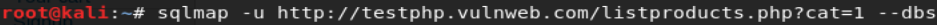
\includegraphics[width=0.8\textwidth]{oui/Screens/Nikto/2.PNG}
  \caption{Scan d'un port}
  \label{fig:courbe-tikz}
\end{figure}

Le port 443 est le port HTTPS que nous allons cibler avec le port 80 :

\begin{figure}[htp!]
  \centering
  \setlength\figureheight{7cm}
  \setlength\figurewidth{9cm}
  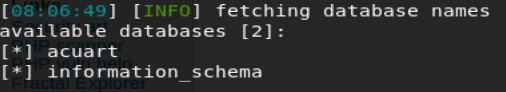
\includegraphics[width=0.8\textwidth]{oui/Screens/Nikto/3.PNG}
  \caption{Scan de plusieurs ports}
  \label{fig:courbe-tikz}
\end{figure}

\newpage
Scan multihosts :


Il est possible de scanner une plage d’adresses de serveurs Web. Nikto est capable de lire sur son entrée standard. Du coup, on lui donne le résultat d’un scan nmap :\\
\begin{center}   
\textbf{nmap -p80 192.168.0.0/24 -oG - | ./nikto -h}
\end{center}

Scan verbeux et debug:

\begin{figure}[htp!]
  \centering
  \setlength\figureheight{7cm}
  \setlength\figurewidth{9cm}
  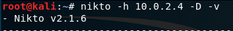
\includegraphics[width=0.8\textwidth]{oui/Screens/Nikto/4.PNG}
  \caption{Commande}
  \label{fig:courbe-tikz}
\end{figure}

\begin{figure}[htp!]
  \centering
  \setlength\figureheight{7cm}
  \setlength\figurewidth{9cm}
  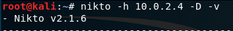
\includegraphics[width=0.8\textwidth]{oui/Screens/Nikto/4.PNG}
  \caption{Résultats}
  \label{fig:courbe-tikz}
\end{figure}

L’option -v permet au terminal d’afficher plus d’éléments sur l’écran afin d’avoir de plus amples connaissances sur la cible.\\
L’option -D permet de corriger les potentiels bugs.\\

Détection du type de serveur Web:

\begin{figure}[htp!]
  \centering
  \setlength\figureheight{7cm}
  \setlength\figurewidth{9cm}
  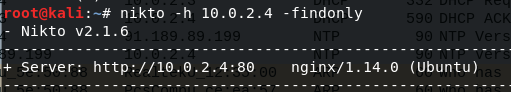
\includegraphics[width=0.8\textwidth]{oui/Screens/Nikto/nikto8.PNG}
  \caption{Détection Serveur Web}
  \label{fig:courbe-tikz}
\end{figure}

Comme nous pouvons le constater grâce à la capture ci-dessus, nikto offre la possiblité de ne détecter que la version du serveur et rien d'autre. 

Gagner en discrétion:

\begin{figure}[htp!]
  \centering
  \setlength\figureheight{7cm}
  \setlength\figurewidth{9cm}
  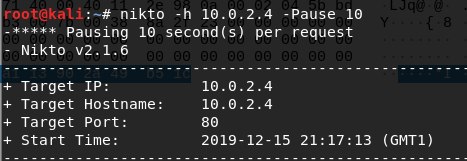
\includegraphics[width=0.8\textwidth]{oui/Screens/Nikto/nikto9.PNG}
  \caption{ajout de l'argument Pause}
  \label{fig:courbe-tikz}
\end{figure}

Cette méthode permettant de diminuer en agressivité et donc de gagner en discrétion lors du scan. En ajoutant l'option -Pause 10, on demande à nikto d'attendre 10 secondes entre deux tests.

\begin{figure}[htp!]
  \centering
  \setlength\figureheight{7cm}
  \setlength\figurewidth{9cm}
  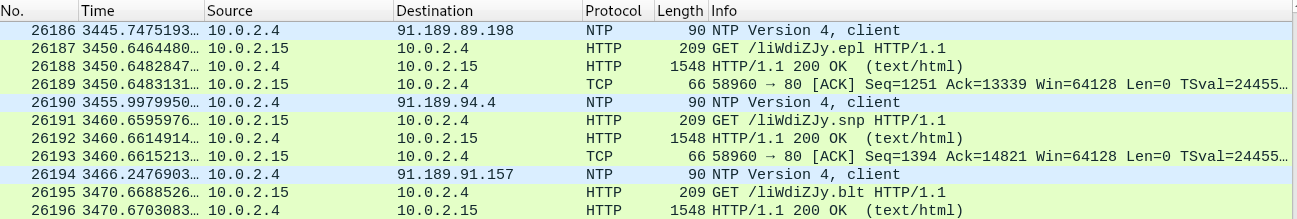
\includegraphics[width=0.8\textwidth]{oui/Screens/Nikto/wireshark4.PNG}
  \caption{Capture wireshark du scan avec l'otpion de pause}
  \label{fig:courbe-tikz}
\end{figure}

On remarque l'utilisation du protocole NTP (Network Time Protocol) qui permet ici de mettre en place le temps de pause.

\noindent \textbf{Avertissement}\\
Nikto ne doit être utilisé uniquement sur ses propres serveurs.En effet, le scan est bruyant, et peut générer plusieurs dizaines de lignes de logs avec votre IP dans les logs apache ou dans n’importe quel IDS (système de détection d’intrusion). L’intérêt de nikto est donc de trouver des failles chez soi pour pouvoir sécuriser au mieux ses propres serveurs web.\\
\noindent \textbf{Conclusion}\\
Nikto est un programme très utile lorsqu'il s'agit de scanner les failles de sécurité de son serveur web et son exécution est assez rapide (suivant l’architecture matérielle de l’hôte).
En revanche, Nikto a le défaut d’être aisément repérable dans les logs et donne donc l’adresse IP de celui qui scanne.
